现在,我们对处理器高效使用的理解是:首先,CPU可以同时做多个操作,比如:同时做加法和乘法。不使用这种能力就是暴殄天物。此外,限制效率最大化能力的因素是,生成数据的速度,以供给这些操作进行计算。受到数据依赖关系的约束:如果一个操作计算了下一个操作用作输入的值,那么这两个操作必须顺序执行。处理这种依赖关系的方法是流水线操作,当执行循环或长的代码序列时,处理器将交叉计算(如循环迭代),只要有可以独立执行的操作即可。

使用流水线也有前提条件。流水线的\textbf{前提条件}:为了从循环迭代中交叉执行代码,必须知道将执行什么代码。与上一节中了解到的信息进行比较,为了并行执行指令,必须预先知道输入值。现在,为了在流水线中运行指令,必须知道指令是什么。现在知道吗?因为运行的代码通常依赖于数据,每次遇到\texttt{if(条件)}语句时,要么执行\texttt{true}分支,要么执行\texttt{false}分支,但是在确定\textit{条件}之前我们并不知道会执行到哪个分支。像数据依赖是指令级并行的障碍一样,条件执行或分支也是流水线的障碍。

随着流水线的中断,程序的效率会显著降低。我们可以使用基准测试来观察这种有害影响,例如不要写这样的代码:

\begin{lstlisting}[style=styleCXX]
a1 += p1[i] + p2[i];
\end{lstlisting}

可以这样写:

\begin{lstlisting}[style=styleCXX]
a1 += (p1[i]>p2[i]) ? p1[i] : p2[i];
\end{lstlisting}

现在我们将数据依赖重新引入到代码中了:

%\hspace*{\fill} \\ %插入空行
\begin{center}
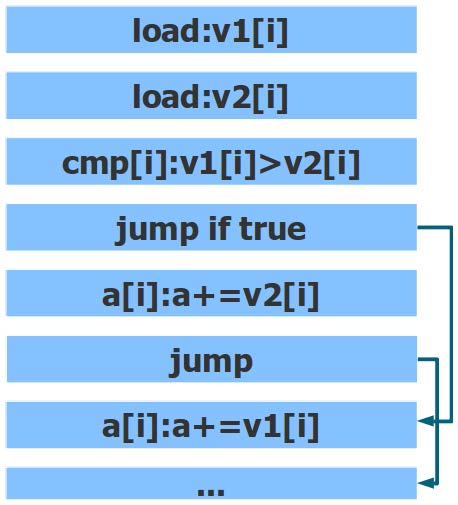
\includegraphics[width=0.4\textwidth]{content/1/chapter3/images/18.jpg}\\
图3.18 - 转移指令对流水线的影响
\end{center}

没有好方法将这段代码转换为要执行的线性指令流,并且需要处理不能避免的条件跳转。

实际情况要复杂一些,基准测试可能会出现性能的显著下降,也可能不会。原因是许多处理器都有某种\textbf{条件移动}功能,甚至是\textbf{条件添加}指令,编译器可以决定是否使用。如果发生这种情况,代码就会变得完全有序,没有跳转或分支,并且可以完美地流水线化:

%\hspace*{\fill} \\ %插入空行
\begin{center}
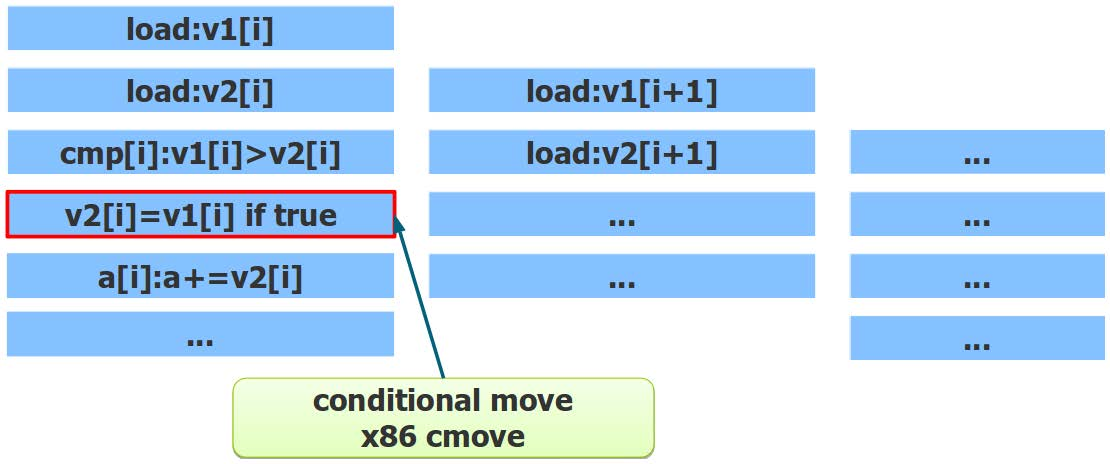
\includegraphics[width=0.9\textwidth]{content/1/chapter3/images/19.jpg}\\
图3.19 - cmove将分支流水线化
\end{center}

x86的CPU有一个条件移动指令\texttt{cmove}(虽然不是所有编译器都使用它来实现\texttt{?:}三元操作符)。具有AVX或AVX2指令集的处理器具有一组强大的掩码加法和乘法指令,这些指令也可以用于实现一些条件代码。这就是为什么在用分支对代码进行基准测试和优化时,需要检查生成的目标代码,并确认代码中确实包含分支,以及确定是否影响了性能。还有一些分析器工具可用,我们稍后介绍。

虽然分支和条件在大多数现实程序中无处不在,但当程序减少到只有几行代码时就会消失,原因是编译器可能使用了前面提到的条件指令。构造糟糕的基准测试的另一个原因是,编译器能够在编译时计算出条件的值,大多数编译器将完全优化代码,比如:\texttt{if (true)}或\texttt{if (false)}生成的代码中就没了这个语句,永远不会执行的代码也会消除。要了解分支对循环流水线的有害影响,必须构造一个编译器无法预测条件检查结果的测试,可以从实际使用的程序中提取了一个数据集。下一个演示,将使用随机值:

\hspace*{\fill} \\ %插入空行
\noindent
\textbf{02\_branch.C}
\begin{lstlisting}[style=styleCXX]
std::vector<unsigned long> v1(N), v2(N);
std::vector<int> c1(N);
for (size_t i = 0; i < N; ++i) {
	v1[i] = rand();
	v2[i] = rand();
	c1[i] = rand() & 1;
}
unsigned long* p1 = v1.data();
unsigned long* p2 = v2.data();
int* b1 = c1.data();
for (auto _ : state) {
	unsigned long a1 = 0, a2 = 0;
	for (size_t i = 0; i < N; ++i) {
		if (b1[i]) {
			a1 += p1[i];
		} else {
			a1 *= p2[i];
		}
	}
	benchmark::DoNotOptimize(a1);
	benchmark::DoNotOptimize(a2);
	benchmark::ClobberMemory();
}
\end{lstlisting}

同样,有两个输入数组\texttt{v1}和\texttt{v2},以及一个随机值为0和1的控制数组\texttt{c1}(这里请避免使用\texttt{vector<bool>},它不是字节数组,而是一个打包的位数组,因此访问它的开销会很高,而且我们现在对位操作指令的基准测试不感兴趣)。编译器无法预测下一个随机数是奇数还是偶数,因此不可能进行优化。此外,我们检查了生成的机器码,并确认编译器(x86上的Clang-11)使用一个简单的条件跳转实现了这个循环。为了有一个基线测试,我们将这个循环的性能与在每次迭代中进行无条件加法和乘法的循环进行比较:\texttt{a1 += p1[i]*p2[i]}。这个简单的循环在每次迭代中都做加法和乘法,由于流水线的存在,我们可以自由地进行加法运算,与下一次迭代的乘法运算同时执行。另一方面,条件分支不能自由的执行:

%\hspace*{\fill} \\ %插入空行
\begin{center}
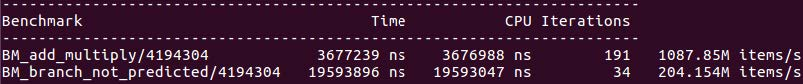
\includegraphics[width=0.9\textwidth]{content/1/chapter3/images/20.jpg}\\
图 3.20
\end{center}

可以看到,条件代码大约比顺序代码慢5倍。证实了我们的预测,当下一条指令依赖于上一条指令的结果时,代码不能有效地流水化。

\subsubsubsection{3.5.1\hspace{0.2cm}分支预测}

聪明的读者可能会指出,我们刚才描述的图像可能不完整,甚至不是真实的。让我们回到串行代码上,例如:我们在上一节中使用的循环代码:

\begin{lstlisting}[style=styleCXX]
for (size_t i = 0; i < N; ++i) {
	a1 += v1[i] + v2[i]; // s[i] = v1[i] + v2[i]
}
\end{lstlisting}

处理器视角的循环体:

%\hspace*{\fill} \\ %插入空行
\begin{center}
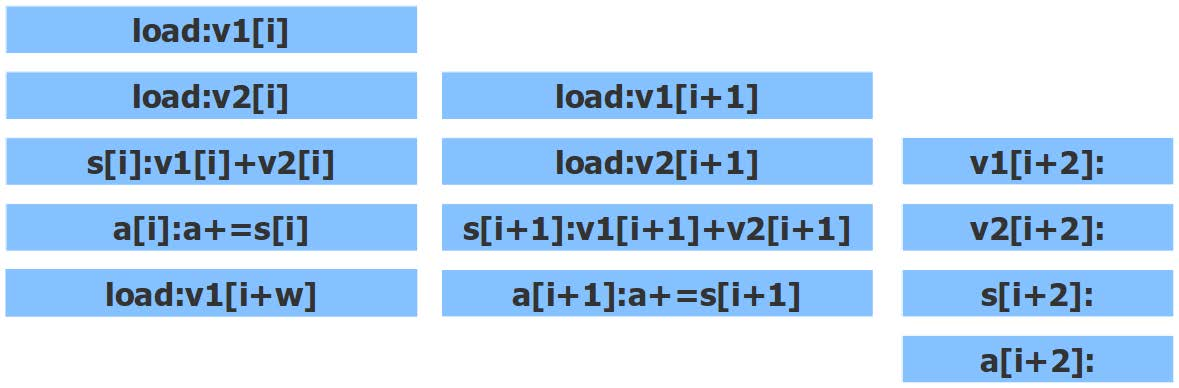
\includegraphics[width=0.8\textwidth]{content/1/chapter3/images/21.jpg}\\
图3.21 - 宽度为w的流水线中执行的循环
\end{center}

图3.21中,展示了三次交叉迭代,但可能有更多,流水线的总宽度是w,理想情况下,w足够大。每个周期中,CPU执行指令都可以同时执行(这样的峰值效率在实际中很少)。但请注意,在计算\texttt{p1[i] + p2[i]}的同时,可能不可能访问\texttt{v[i+2]},因为不能保证循环有更多的两次迭代,所以\texttt{v[i+2]}可能不存在,贸然访问会导致未定义行为。前面代码中有一个隐藏条件:每次迭代中,必须检查i是否小于N,只有这样才能执行第i次迭代的指令。

因此,在图3.20中的比较是错误的,没有将流水线的顺序执行与不可预测的条件执行进行比较。实际上,这两个基准测试都有分支。

真相介于两者之间,我们了解条件执行的解决方案。流水线是数据依赖的解决方案,但分支戕害了它。分支存在时,保存流水线的方法是尝试将条件代码转换为顺序代码,如果事先知道分支要走哪条路,就可以进行转换。只需消除分支,然后继续执行下一条指令。当然,如果事先知道情况如何,就没必要这样写代码了。这里,考虑一下循环的终止条件。假设循环执行了很多次,可能条件\texttt{i < N}的计算结果为\texttt{true}(只有\texttt{1 / N}的几率会输掉这个赌局)。

处理器使用\textbf{分支预测}技术进行押注。分析代码中每一个分支的历史,并假定该行为在未来不会变。循环结束后,处理器很快就会知道,大多数情况下,必须进行下一个迭代。因此,正确的做法是对下一次迭代进行流水线化。当然,必须将实际的结果写入内存,直到计算条件确认迭代确实发生。处理器有一定数量的写缓冲区来保存这些未确认的结果,然后再将它们提交到内存中。

因此,只添加了一个元素的循环流水,看起来与图3.21所示完全一致。唯一的问题是,当第\texttt{i}次迭代完成之前开始执行迭代\texttt{i+2}时,处理器根据是否采用条件分支预测来下注的。这种确定代码存在的执行方式,称为\textbf{投机执行}。赌赢了,知道需要计算的时候,就可以获取结果。如果输了,必须放弃一些计算结果,以避免产生错误,例如:写入内存新内容,覆盖之前的内容,在大多数硬件平台上无法撤消,而计算结果和将其存储在寄存器中的过程完全可逆。当然,这会浪费我们的时间。

现在我们对流水线的工作原理有了更全面的了解。为了找到更多的指令并行执行,处理器要检查循环的下一个迭代,并开始与当前迭代同时执行。该代码包含一个条件分支,无法确切地知道将执行哪条指令,处理器根据过去检查的结果进行有根据的猜测,并继续推测执行该代码。若这个预测正确,则流水线操作可以和无条件代码一样好。若预测错误,处理器必须丢弃预测得到的结果,获取之前认为不需要的指令,并进行计算。这个事件称为\textbf{刷新流水},是一个开销很大的事件。

现在对图3.20中的基准测试有了更好的理解,两个循环都有检查循环结束的条件。然而,预测几乎是完美的,刷新流水只在循环的末端发生。条件基准测试也有基于随机数的分支,\texttt{if(b1[i])},其中\texttt{b1[i]}有50\%的概率为真。处理器无法预测结果,并且一半的时间流水中断了(或者更糟,如果设法欺骗了CPU,会使其做出了错误的预测)。

可以用实验来验证我们的理解,只需要把随机条件改变成总是正确即可。唯一的问题是,我们必须以编译器无法理解的方式来处理。常用的方法是将条件数组进行初始化:

\begin{lstlisting}[style=styleCXX]
c1[i] = rand() >= 0;
\end{lstlisting}

编译器不知道函数\texttt{rand()}总是返回非负的随机数,并且不会消除这种情况。CPU的分支预测器电路很快就会知道,如果\texttt{if(b1[i])}的值总是为真,那么就会推测地执行相应的代码。我们可以良好的预测分支和不准确预测分支的性能:

%\hspace*{\fill} \\ %插入空行
\begin{center}
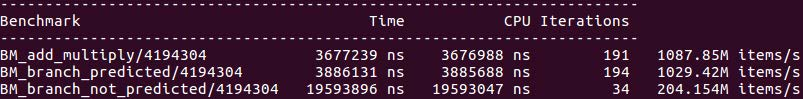
\includegraphics[width=0.9\textwidth]{content/1/chapter3/images/22.jpg}\\
图 3.22
\end{center}

我们可以看到,良好预测分支的成本很低。

\subsubsubsection{3.5.2\hspace{0.2cm}错误预测分支的分析}

已经看到错误预测分支会对代码性能产生多么严重的影响,现在的问题是,如何找到这样的代码来优化?当然,包含这段代码的函数所花费的时间比预期的要长,但是如何知道其原因是因预测错误的分支,还是其他原因才效率低下的呢?现在,我们已经了解了足够多的知识,从而可以\textit{避免对性能的猜测},且猜测分支预测器的有效性挺没趣的。通常,大多数分析器不仅可以分析执行时间,还可以分析决定效率的各种因素,包括分支预测失败。

本章中,将再次使用perf分析器。第一步,运行这个分析器来收集基准程序的总体性能指标:

\begin{tcblisting}{commandshell={}}
$ perf stat ./benchmark
\end{tcblisting}

下面是只运行\texttt{BM\_branch\_not\_predicted}基准测试的性能结果(其他基准测试注释掉了):

%\hspace*{\fill} \\ %插入空行
\begin{center}
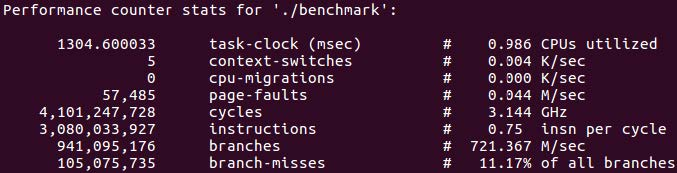
\includegraphics[width=0.9\textwidth]{content/1/chapter3/images/23.jpg}\\
图3.23 - 预测分支失败的基准测试数据
\end{center}

11\%的所有分支被预测错误(报告的最后一行)。请注意,这个数字是所有分支的累加,包括完全可预测的循环结束条件,因此11\%相当糟糕。我们应该将它与其他基准\texttt{BM\_branch\_predicted}进行比较,\texttt{BM\_branch\_predicted}和这个基准测试完全相同,只是条件总是为真:

%\hspace*{\fill} \\ %插入空行
\begin{center}
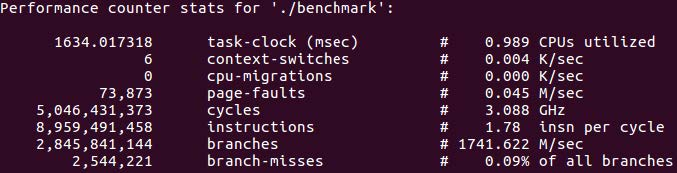
\includegraphics[width=0.9\textwidth]{content/1/chapter3/images/24.jpg}\\
图3.24 - 具有预测良好分支的基准测试概要
\end{center}

这一次,不到0.1\%的分支没有正确预测。

报告非常有用,可以用来强调或消除一些可能导致不良表现的原因。我们的案例中,可以得出结论,程序有一个或多个错误预测的分支。现在只需要找到是哪一个,分析器也可以帮忙查找。上一章中,使用分析器找出程序花费时间最多的地方,可以生成分支预测的逐行数据。我们只需要为分析器指定正确的性能计数器即可:

\begin{tcblisting}{commandshell={}}
$ perf record -e branches,branch-misses ./benchmark
\end{tcblisting}

我们的例子中,可以从\texttt{perf stat}的输出复制计数器的名称,因为它恰好是默认测量的计数器之一,完整的列表可以通过运行\texttt{perf -\,-list}获得。

分析器运行程序并收集指标,可以通过生成数据报告来查看:

\begin{tcblisting}{commandshell={}}
$ perf report
\end{tcblisting}

报表分析器是交互式的,可以导航到每个函数的分支错误预测计数器:

%\hspace*{\fill} \\ %插入空行
\begin{center}
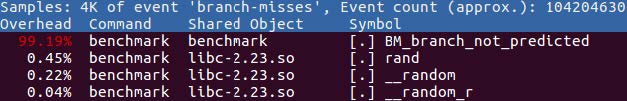
\includegraphics[width=0.9\textwidth]{content/1/chapter3/images/25.jpg}\\
图3.25 - 错误预测分支的详细报告
\end{center}

超过99\%的错误预测分支发生在一个函数中。因为函数很小,所以查找相应的条件运算应该不难。在更大的函数中,我们必须逐行查看概要信息。

现代处理器的分支预测硬件相当复杂,例如:函数从两个不同的位置调用,当从第一个位置调用时,条件的计算结果为true,而从第二个位置调用时,相同的条件的计算结果为false,预测器会了解该模式,并根据函数调用正确地预测分支。类似地,预测器可以在数据中检测出相当复杂的模式,例如:可以初始化我们的随机条件变量,使值总是不可预测的,第一个是随机的,但是下一个是与第一个相反的,以此类推:

\begin{lstlisting}[style=styleCXX]
for (size_t i = 0; i < N; ++i) {
	if (i == 0) c1[i] = rand() >= 0;
	else c1[i] = !c1[i - 1];
}
\end{lstlisting}

分析器确认该数据的分支预测率非常好:

%\hspace*{\fill} \\ %插入空行
\begin{center}
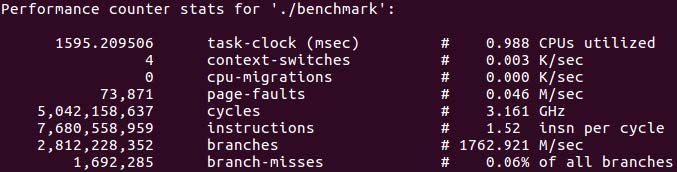
\includegraphics[width=0.9\textwidth]{content/1/chapter3/images/26.jpg}\\
图3.26 - “真-假”模式的分支预测率
\end{center}

我们已经准备好如何高效使用处理器了。但必须承认,这里忽略了一个很重要的问题。































